\newpage
\section{Part B}

\begin{figure}[htbp]
   \centering
   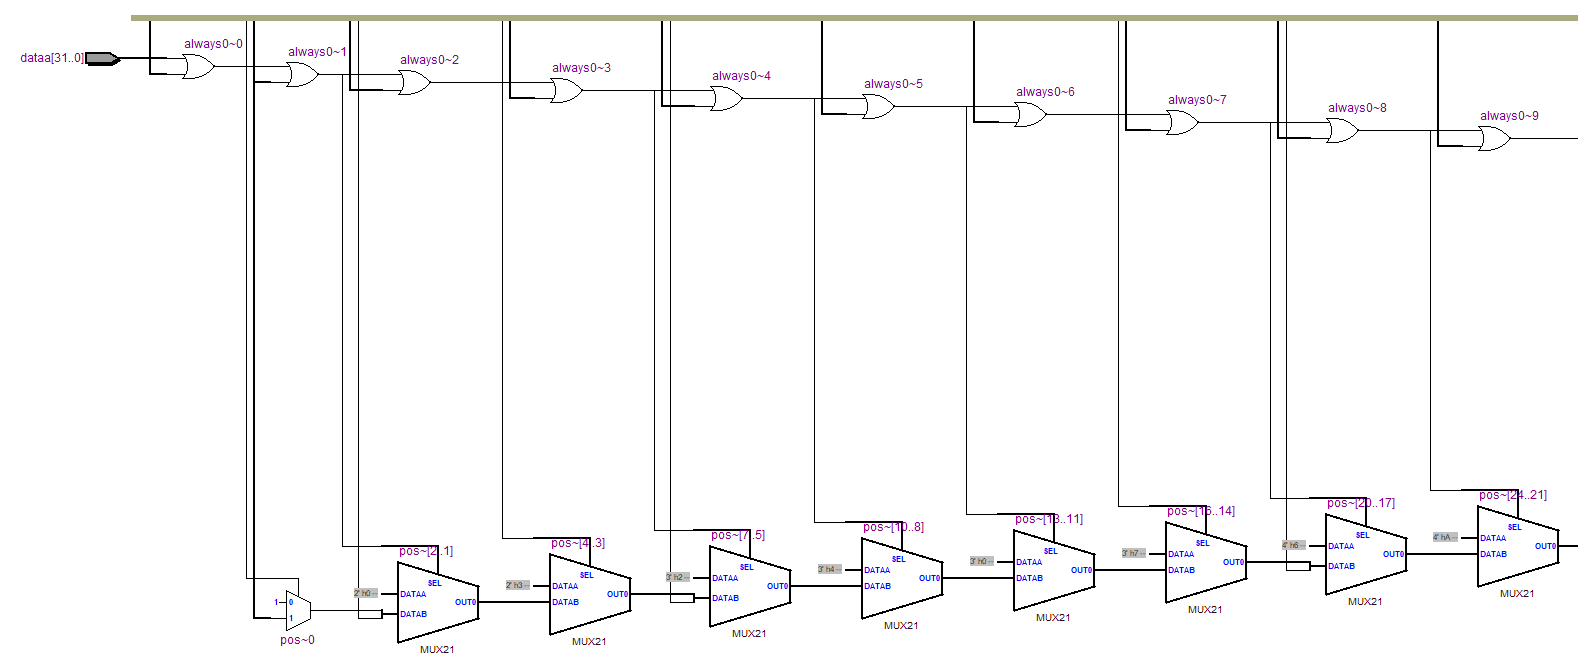
\includegraphics[width=\textwidth]{clz-partial-hw}
   \caption{Partial view of the hardware implementation of the clz instruction}
   \label{fig:clz-partial-hw}
\end{figure}

\begin{figure}[htbp]
   \centering
   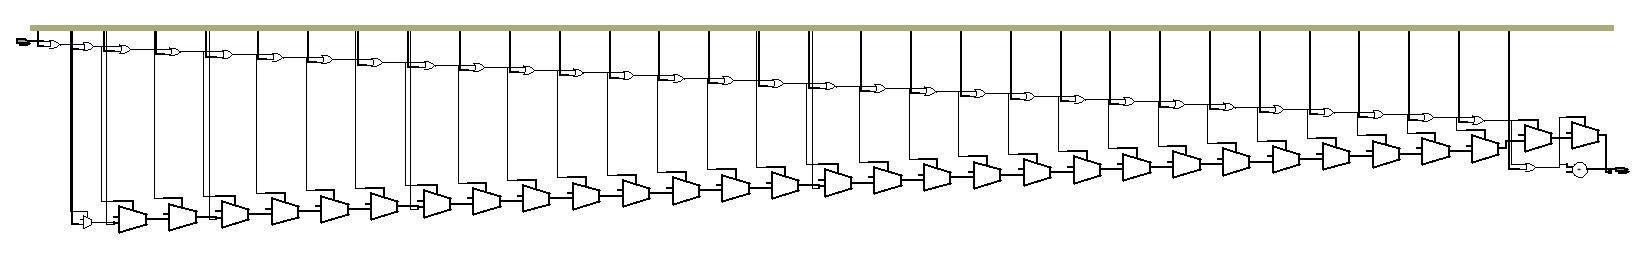
\includegraphics[width=\textwidth]{clz-hw}
   \caption{Rough schematic of the hardware implementation of the clz instruction}
   \label{fig:clz-hw}
\end{figure}

\begin{figure}[htbp]
   \centering
   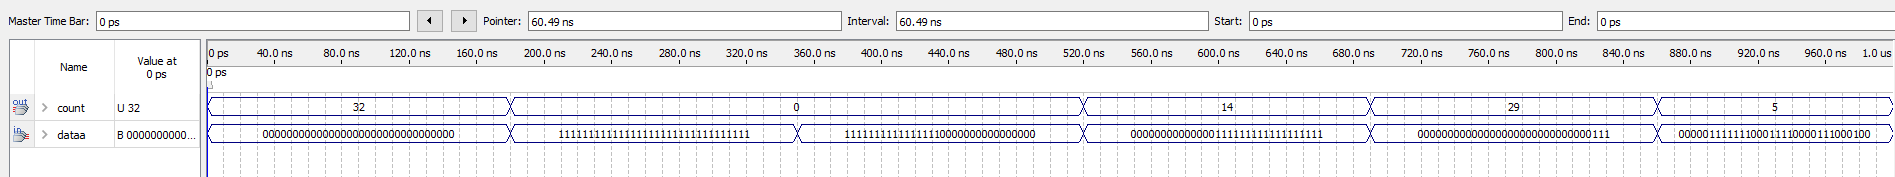
\includegraphics[width=\textwidth]{functional-sim}
   \caption{Functional simulation results of the clz instruction}
   \label{fig:functional-sim}
\end{figure}

\begin{figure}[htbp]
   \centering
   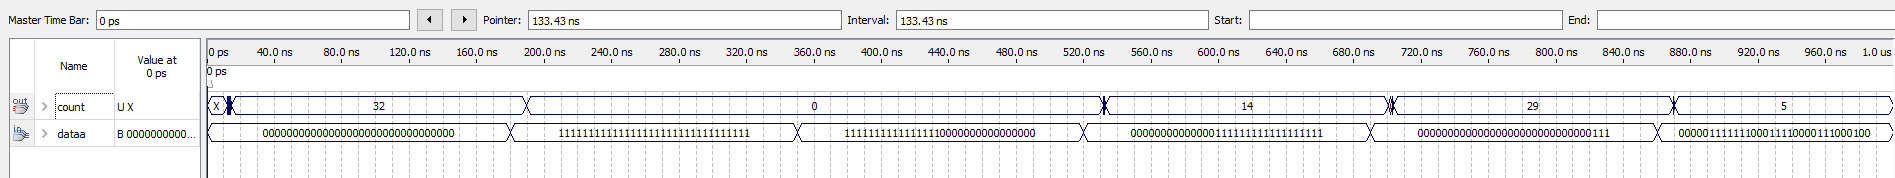
\includegraphics[width=\textwidth]{timing-sim}
   \caption{Timing simulation results of the clz instruction}
   \label{fig:timing-sim}
\end{figure}

Figure \ref{fig:clz-partial-hw} and \ref{fig:clz-hw} are the schematic of the hardware implementation of the count leading zero (clz) instruction. The implementation is a series of multiplexers and OR gates. Figure \ref{fig:functional-sim} and \ref{fig:timing-sim} are the simulation test results of the implementation, which shows it is functioning correctly.

\begin{figure}[htbp]
   \centering
   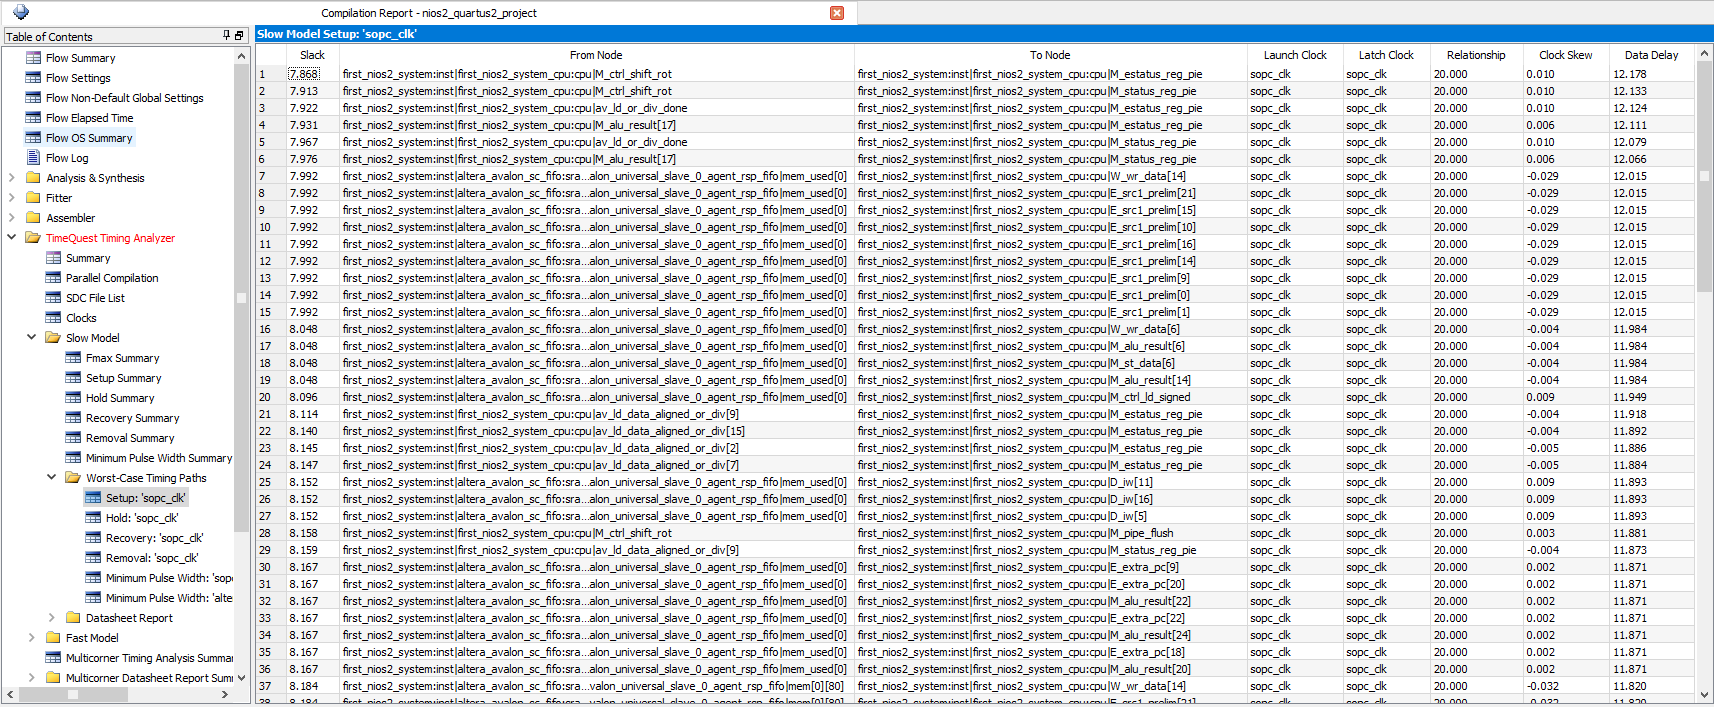
\includegraphics[width=\textwidth]{slowest-data-delay}
   \caption{Slowest data delay of the system}
   \label{fig:}
\end{figure}

\begin{figure}[htbp]
   \centering
   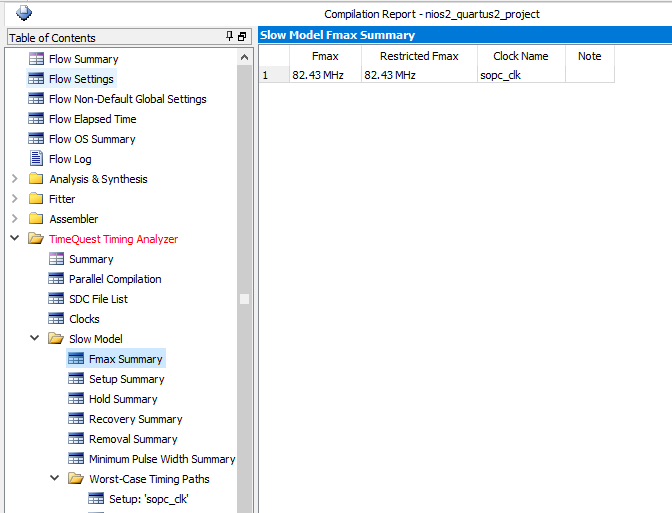
\includegraphics[width=\textwidth]{max-frequency}
   \caption{Maximum frequency of the system}
   \label{fig:}
\end{figure}

After adding the custom instruction, clz, to the system, the slowest data delay is 12 nanoseconds. The maximum frequency the system could reach is 82 MHz, which satisfies the requirement, 50 MHz.

For fair comparison between the hardware implementation and software implementation, the optimisation level was set to O3 for the best performance, as shown in Figure \ref{fig:O3-enabled-for-fair-comparison}. The empirical result, as demonstrated in Figure \ref{fig:part-b}, shows that the hardware implementation of the count leading zero is much faster than the software implementation which is a builtin function of GCC.

\begin{figure}[htbp]
   \centering
   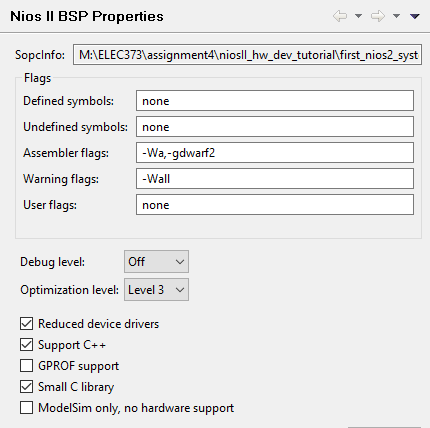
\includegraphics[width=\textwidth]{O3-enabled-for-fair-comparison}
   \caption{O3 enabled for fair comparison}
   \label{fig:O3-enabled-for-fair-comparison}
\end{figure}

\begin{figure}[htbp]
   \centering
   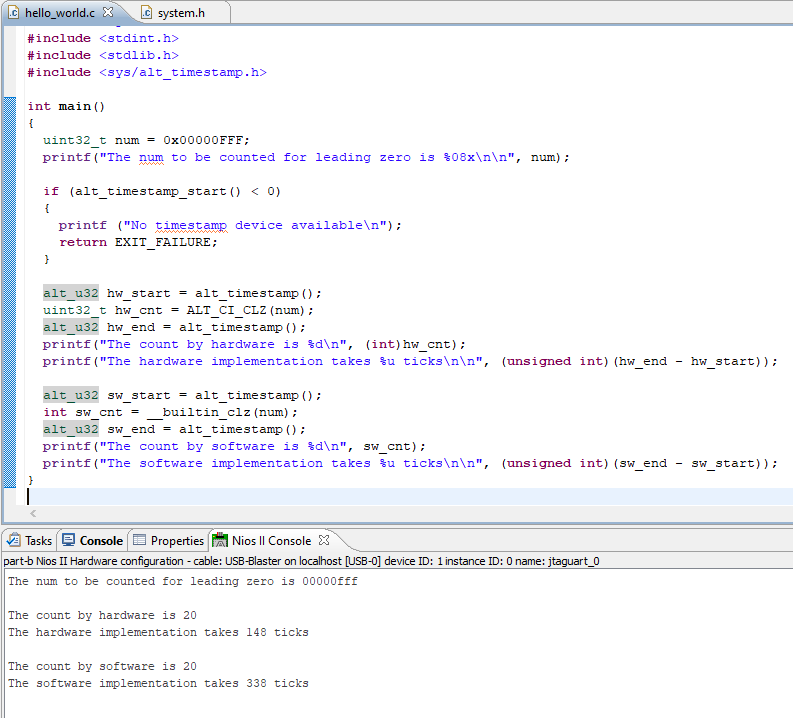
\includegraphics[width=\textwidth]{part-b}
   \caption{The hardware implementation is faster than the software implementation}
   \label{fig:part-b}
\end{figure}
